
\documentclass{article}

\def\mytitle{AnnBrCaPaper}
\def\myauthor{Arindam Bose}

\section{The Work so Far }
\label{theworksofarpreliminaryanalyses}

\begin{document}

Data from the spreadsheet was abstracted and a new data table was created that contained the following information:

\begin{enumerate}
\item The name of the country where the screening for breast cancer,

\item The percentage reduction in the usage of HRT between peak use and the last reported use

\item The percentage reduction in the reported incidence for the corresponding years for the relevant age groups (50--64+)

\item The Age Range at which Screening for Breast Cancer using Mammograms begin. If the age range was 50--64 years, it was given a code of 1, else if the age at which mammogram began was earlier (that is for younger age), the Age range variable was assigned a code of 2.

\end{enumerate}

In addition to this, data from the papers by Verkooijen et al (Verkooijen, Bouchardy, Vinh-Hung, Rapiti, \& Hartman, 2009) and Zbuk et al (Zbuk \& Anand, 2012) were extracted. For each of these data, the following information were abstracted from each paper

\begin{enumerate}
\item The name of the country where the study was conducted

\item The percentage of reduction from peak HRT usage till the date when it was reported

\item The reduction in percentage in the corresponding breast cancer incidence as reported in the paper.

\end{enumerate}

These were presented in a corresponding table abstracted from the papers (see Figures 1 and 2). For each of the three data, a linear regression model was run to study the extent to which reduction in the HRT usage might explain the reduction in the incidence of Breast Cancer. For the current dataset, in addition, the relationship between the reduction in Breast Cancer and the HRT usage was further adjusted for by including the age at which screening begins. 

\section*{Results}
\label{results}

Table 1 shows the data abstracted from the current dataset.

\begin{table}[htbp]
\begin{minipage}{\linewidth}
\setlength{\tymax}{0.5\linewidth}
\centering
\small
\begin{tabulary}{\textwidth}{@{}LLLL@{}} \toprule
Country&Reduction in HRT Usage (pct)&Reduction in Br Ca (percent)&Age Category of Screening\\
\midrule
Australia&43&6.7&40--75\\
Canada&70&8&50--69\\
Denmark&19&5.63&50--69\\
France&66&6.3&50--69\\
Italy&42&6.18&50--69\\
United States&33&6.7&40--75\\
Germany&50&8.8&40--75\\
Belgium&60&9.5&50--69\\

\bottomrule

\end{tabulary}
\end{minipage}
\end{table}


\includegraphics[keepaspectratio,width=\textwidth,height=0.75\textheight]{ourdata.jpg}

Figure 1 shows the graph from the regression model of the relationship between reduction in HRT usage and reduction in breast cancer incidence from the studies included in this paper

Exhibit 1 shows the results of the regression model from the data abstracted for this analysis.
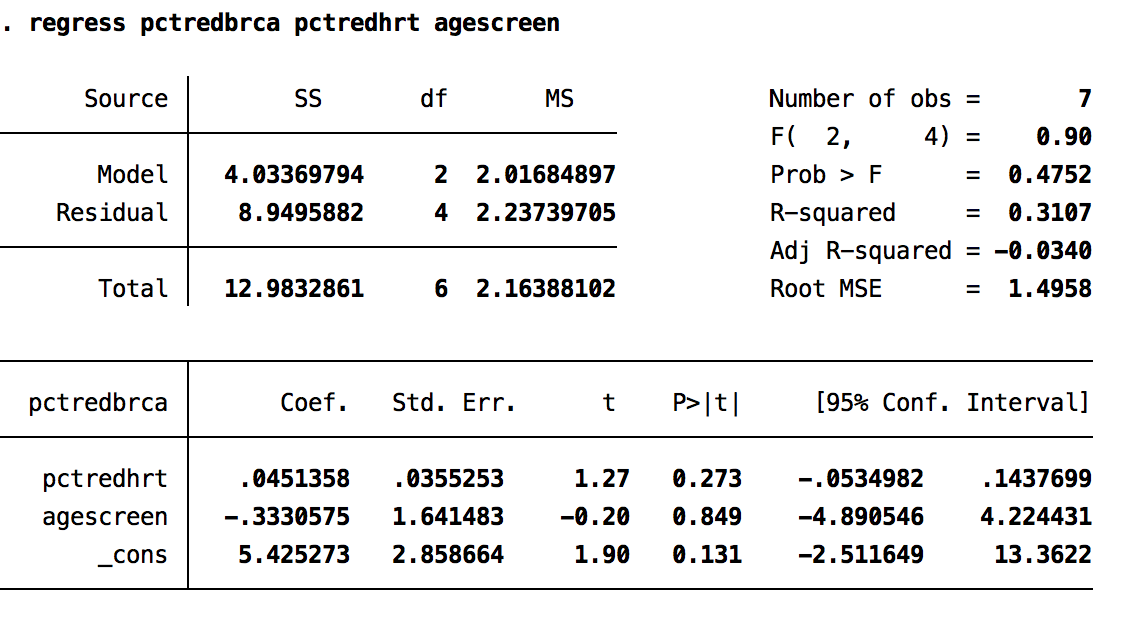
\includegraphics[keepaspectratio,width=\textwidth,height=0.75\textheight]{ourfigure.png}


\section*{Comparison with Two Other Studies (Zbuk and Anand and Verkooijen et al)}
\label{comparisonwithtwootherstudieszbukandanandandverkooijenetal}

For comparison, we present two other datasets and two other analyses, one from the paper by Zbuk and Anand and the other by a paper by Verkooijen. 

Figure 2. Data from the paper by Zbuk
\includegraphics[keepaspectratio,width=\textwidth,height=0.75\textheight]{zbuk.jpg}


Figure 3 presents the results of data analyses and regression model constructed from the zbuk data.
\includegraphics[keepaspectratio,width=\textwidth,height=0.75\textheight]{zbukgraph.jpg}


Figure 4 presents the regression outputs from the Zbuk data abstracted from the paper
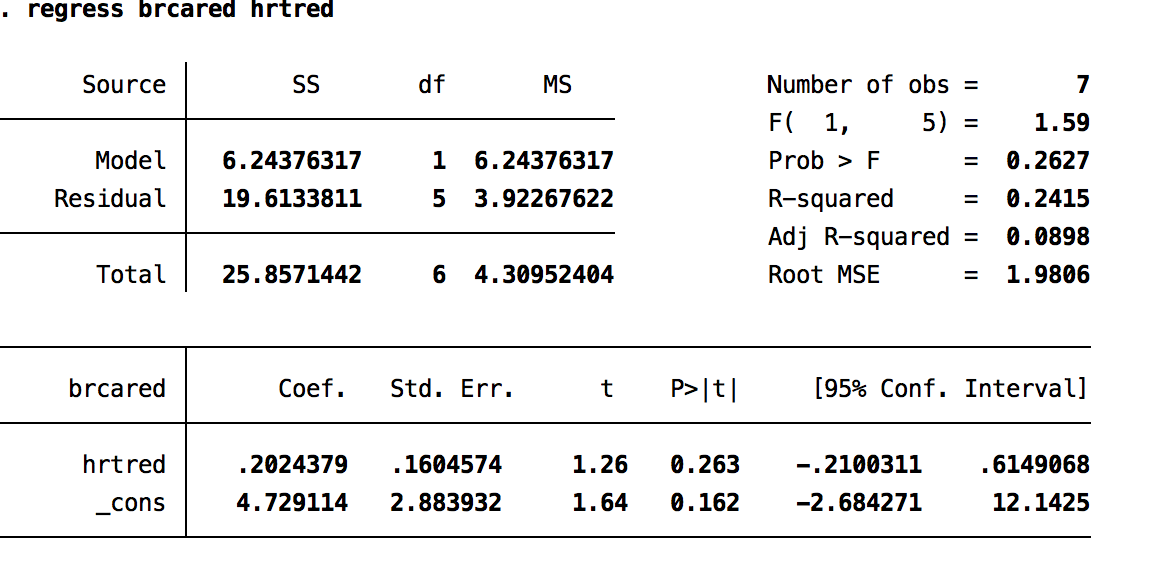
\includegraphics[keepaspectratio,width=\textwidth,height=0.75\textheight]{zbukoutput.png}


Figure 5 presents the tables from Verkooijen study
\includegraphics[keepaspectratio,width=\textwidth,height=0.75\textheight]{verkooijen.jpg}


Figure 6 presents the figure of the data analyses from regression model constructed from Verkooijen study
\includegraphics[keepaspectratio,width=\textwidth,height=0.75\textheight]{verkgraph.jpg}


Figure 7 presents the figure of the regression table from Verkooijen study
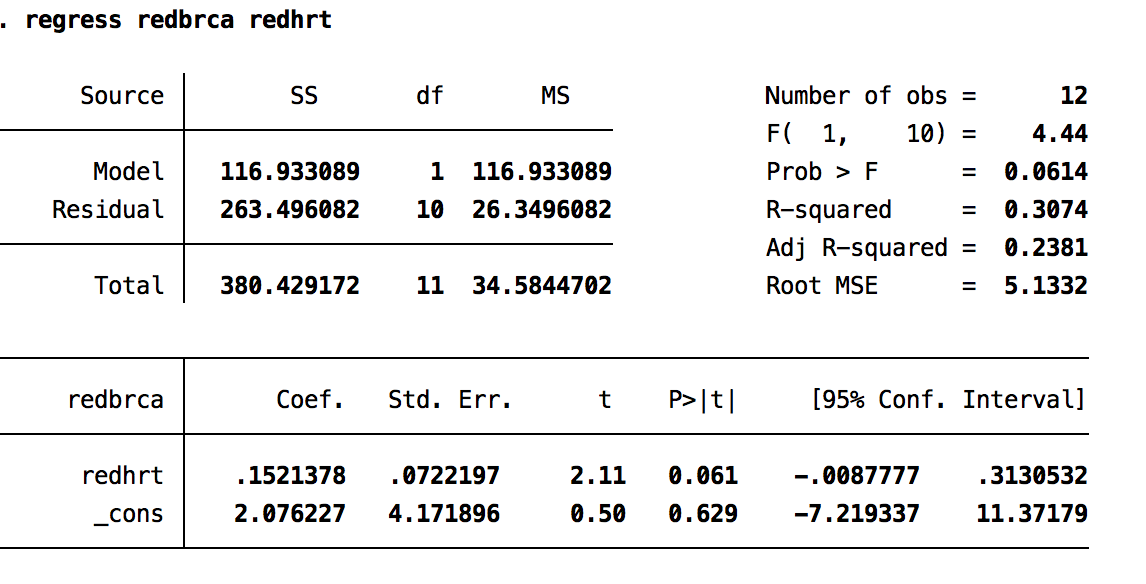
\includegraphics[keepaspectratio,width=\textwidth,height=0.75\textheight]{verkoutput.png}


\section*{Reference}
\label{reference}

Verkooijen, H. M., Bouchardy, C., Vinh-Hung, V., Rapiti, E., \& Hartman, M. (2009). The incidence of breast cancer and changes in the use of hormone replacement therapy: A review of the evidence. Maturitas, 64(2), 80--5. doi:10.1016\slash j.maturitas.2009.07.015

Zbuk, K., \& Anand, S. S. (2012). Declining incidence of breast cancer after decreased use of hormone-replacement therapy: Magnitude and time lags in different countries. Journal of Epidemiology and Community Health, 66(1), 1--7. doi:10.1136\slash jech.2008.083774
\end{document}
